\documentclass[border=10pt]{standalone}
\usepackage{tikz}
\usepackage{xcolor}
\usetikzlibrary{shapes, arrows.meta, calc, positioning}

% --- Paleta de colores ---
\definecolor{azulBorde}{HTML}{1971c2}
\definecolor{azulFondo}{HTML}{a5d8ff}
\definecolor{verdeBorde}{HTML}{2f9e44}
\definecolor{verdeFondo}{HTML}{b2f2bb}
\definecolor{naranjaBorde}{HTML}{e8590c}
\definecolor{naranjaFondo}{HTML}{ffd8a8}
\definecolor{verdeclaroBorde}{HTML}{66a80f}
\definecolor{verdeclaroFondo}{HTML}{d8f5a2}
\definecolor{naranjaclaroBorde}{HTML}{f76707}
\definecolor{naranjaclaroFondo}{HTML}{ffe8cc}

\begin{document}
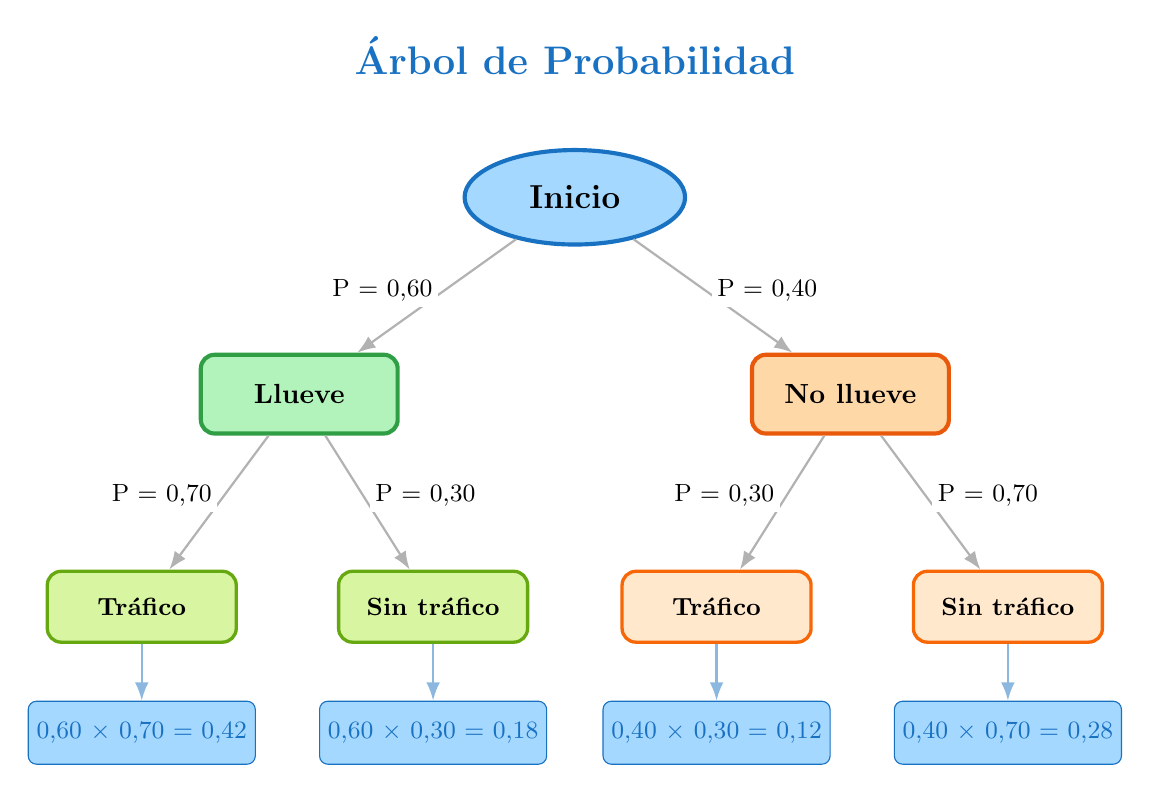
\begin{tikzpicture}[
  % Estilos de nodos
  nodoInicio/.style={
    ellipse, draw=azulBorde, fill=azulFondo,
    line width=1.5pt, font=\bfseries\large,
    minimum width=2.8cm, minimum height=1.2cm
  },
  nodoLlueve/.style={
    rectangle, rounded corners=5pt,
    draw=verdeBorde, fill=verdeFondo,
    line width=1.5pt, font=\bfseries,
    minimum width=2.5cm, minimum height=1cm
  },
  nodoNoLlueve/.style={
    rectangle, rounded corners=5pt,
    draw=naranjaBorde, fill=naranjaFondo,
    line width=1.5pt, font=\bfseries,
    minimum width=2.5cm, minimum height=1cm
  },
  nodoHojaVerde/.style={
    rectangle, rounded corners=5pt,
    draw=verdeclaroBorde, fill=verdeclaroFondo,
    line width=1.2pt, font=\small\bfseries,
    minimum width=2.4cm, minimum height=0.9cm
  },
  nodoHojaNaranja/.style={
    rectangle, rounded corners=5pt,
    draw=naranjaclaroBorde, fill=naranjaclaroFondo,
    line width=1.2pt, font=\small\bfseries,
    minimum width=2.4cm, minimum height=0.9cm
  },
  nodoProb/.style={
    rectangle, rounded corners=3pt,
    draw=azulBorde, fill=azulFondo,
    font=\small, text=azulBorde,
    minimum width=2.8cm, minimum height=0.8cm,
    inner sep=3pt
  },
  % Estilo de flechas
  flecha/.style={
    -Latex, thick, draw=gray!60
  },
  etiqProb/.style={
    font=\small, fill=white, inner sep=2pt
  }
]

% --- Título ---
\node[font=\Large\bfseries, text=azulBorde]
  (titulo) at (5, 1.8) {\'{A}rbol de Probabilidad};

% --- Nodo raíz ---
\node[nodoInicio] (inicio) at (5, 0) {Inicio};

% --- Nivel 1 ---
\node[nodoLlueve]   (llueve)   at (1.5, -2.5) {Llueve};
\node[nodoNoLlueve] (nollueve) at (8.5, -2.5) {No llueve};

% --- Nivel 2 desde Llueve ---
\node[nodoHojaVerde] (trafL)    at (-0.5, -5.2) {Tr\'{a}fico};
\node[nodoHojaVerde] (notrafL)  at ( 3.2, -5.2) {Sin tr\'{a}fico};

% --- Nivel 2 desde No llueve ---
\node[nodoHojaNaranja] (trafNL)   at (6.8, -5.2) {Tr\'{a}fico};
\node[nodoHojaNaranja] (notrafNL) at (10.5, -5.2) {Sin tr\'{a}fico};

% --- Probabilidades finales (cajas azules debajo de hojas) ---
\node[nodoProb] (pf1) at (-0.5, -6.8) {0,60 $\times$ 0,70 = 0,42};
\node[nodoProb] (pf2) at ( 3.2, -6.8) {0,60 $\times$ 0,30 = 0,18};
\node[nodoProb] (pf3) at ( 6.8, -6.8) {0,40 $\times$ 0,30 = 0,12};
\node[nodoProb] (pf4) at (10.5, -6.8) {0,40 $\times$ 0,70 = 0,28};

% --- Flechas Inicio → Nivel 1 ---
\draw[flecha] (inicio) -- (llueve)
  node[etiqProb, pos=0.45, left=2pt] {P = 0,60};
\draw[flecha] (inicio) -- (nollueve)
  node[etiqProb, pos=0.45, right=2pt] {P = 0,40};

% --- Flechas Llueve → Hojas ---
\draw[flecha] (llueve) -- (trafL)
  node[etiqProb, pos=0.45, left=2pt] {P = 0,70};
\draw[flecha] (llueve) -- (notrafL)
  node[etiqProb, pos=0.45, right=2pt] {P = 0,30};

% --- Flechas No llueve → Hojas ---
\draw[flecha] (nollueve) -- (trafNL)
  node[etiqProb, pos=0.45, left=2pt] {P = 0,30};
\draw[flecha] (nollueve) -- (notrafNL)
  node[etiqProb, pos=0.45, right=2pt] {P = 0,70};

% --- Flechas Hojas → Probabilidades finales ---
\draw[flecha, draw=azulBorde!50] (trafL)    -- (pf1);
\draw[flecha, draw=azulBorde!50] (notrafL)  -- (pf2);
\draw[flecha, draw=azulBorde!50] (trafNL)   -- (pf3);
\draw[flecha, draw=azulBorde!50] (notrafNL) -- (pf4);

\end{tikzpicture}
\end{document}

